\chapter{A Sparse Introduction to Compressive Sensing}
\label{sec:basic_cs}

We will introduce the basic idea of compressive sensing with an example quite similar to the one found in \cite{bryan13makingdo}. Suppose we have 100 coins. We suspect that a few of them might be counterfeit, and thus have a slightly different weight than the normal coins. 

The naive approach to finding these coins would be to weigh every one of them with an electric weight, and detect the coins that are off. In other words, we would have to do as many measurements as there are coins. But what if we weighed more than one coin at a time?

Suppose, to the contrary, that we would include 50 coins in every weighing. The recorded weight would be the sum of all the included coins. Would we be able to make do with less weighings than 100? Say if we for example made 20 measurements, and recorded only the deviation from the expected weight. This would lead to the following system of equations:
\[
	\A\x = \y
\]
Here $ \A \in \R^{20 \times 100} $ is a matrix where each row corresponds to one weighing, and the elements $ a_{i,j} $ is either $ 0 $ or $ 1 $, depending on whether coin $ j $ was included in weighing $ i $ or not. The vector $ \y \in \R^{20} $ is our measurement vector, and $ \x \in \R^{100} $ is the solution to our problem. 

Unfortunately, since $ \A $ has far more columns than rows, this system is underdetermined, meaning that solving this system the old-fashioned way yields an infinite set of solutions. 

Here comes the key idea of compressive sensing: we will assume that our solution vector $ \x $ is \textit{sparse}. In our example it would make sense to assume that most coins are not counterfeit, so the solution vector $ \x $ (consisting of deviations from the expected weight) would mostly have elements equal to $ 0 $. Hence, we want to choose the solution from the solution space of $ \A\x = \y $ with the smallest amount of non-zero elements.

The rest of this chapter will consider some of the properties we need of $ \A $ in order to make sure that this procedure works for all $ s $-sparse vectors. 







\section{The General Setting}
As we now have seen, if we assume that our solution vector $ \x $ is the sparsest solution $ \z $ to the system of equations $ \A\z = \y $, there is hope to find a unique solution even though our system of equations is underdetermined. In \cref{sec:minimum_measurements} we will look at when we have unique solutions up to a given sparsity $ s $, but for now we will only consider that minimizing the number of non-zero elements will reduce the solution space drastically. Formally we can write this as an optimization problem as follows:

\begin{equation}
	\minimize{\z \in \Cx^{N}} \norm{\z}_0
	\subjectto \A\z = \y
	\tag{P$_0$}
	\label{eq:P0}
\end{equation}

However, this problem seems to be intractable in practice. It is, in fact, NP-hard in general. A proof of the NP-hardness of \eqref{eq:P0} is found in Section~2.3 of \cite{foucart13intro}, and is obtained by reducing \eqref{eq:P0} to the \textit{exact cover by 3-sets} problem, which is known to be NP-complete.





\subsection{Basis Pursuit}
Since \eqref{eq:P0} is computationally hard, we need something to approximate it. One intuitive guess would be to use minimization of another norm, like the $ \ell_{1} $ or $ \ell_{2} $ norm. It turns out that this is what we usually do in practice. 

The question then becomes, which norm do we use? It can be shown that  as $ p $ gets lower, the $ \ell_{p} $ norm approximates the $ \ell_{0} $ norm better \cite[Section 4.1]{foucart13intro}. We will use the lowest value for $ p $ possible, while still having a minimization problem that can be solved in polynomial time. Thus, we will use the $ \ell_{1} $-norm. \cref{fig:l1l2balls} illustrates why $ \ell_{1} $-minimization works well to find the $ \ell_{0} $ minimum. 


We will illustrate this with an example:

\begin{example} \label{ex:l1l2min}
Let
\[ 
	\A = \begin{bmatrix}1 & 2\end{bmatrix} \quad \y = 2
\]
We want to find the solution $ \z $ to $ \A\z = \y $ that minimizes the $ \ell_{0} $ norm, but to do this we will use the $ \ell_{1} $ and $ \ell_{2} $ norms.

The solution space to $ \A\z = \y $ yields a line in $ \R^{2} $. Intuitively, we can visualize finding the solution to $ \A\z = \y $ that minimizes the $ \ell_{p} $-norm, as having a $ \ell_{p} $-ball $ B_{p}(\0, r) $ centered at the origin, and increasing the radius $ r $ until it intersects with this solution space. The intersection is then the optimal solution. This is what we have shown in \cref{fig:l1l2balls}.

The result of $ \ell_{1} $-minimization gives $ \z = (1, 0) $, which is the correct $ \ell_{0} $ minimum. The result of $ \ell_{2} $-minimization gives $ \z \approx (0.39419, 0.8029) $, which not the correct $ \ell_{0} $ minimum. 
\end{example}
\begin{figure}[t]
	%	\hrule\vspace{10pt}
	\centering
	\begin{tikzpicture}[line cap=round,line join=round,>=triangle 45,x=2.0cm,y=2.0cm, scale=0.8]
\draw[-,color=black] (-1.2,0) -- (1.2,0);
\foreach \x in {-1,-0.5,0.5,1}
\draw[shift={(\x,0)},color=black] (0pt,2pt) -- (0pt,-2pt) node[below] {\color{gray} \tiny $\x$};
\draw[-,color=black] (0,-1.2) -- (0,1.2);
\foreach \y in {-1,-0.5,0.5,1}
\draw[shift={(0,\y)},color=black] (2pt,0pt) -- (-2pt,0pt) node[left] {\color{gray} \tiny $\y$};
\draw[color=black] (0pt,-10pt) node[right] {\color{gray} \tiny $0$};
\clip(-1.2,-1.2) rectangle (1.2,1.2);
\draw [dash pattern=on 1pt off 1pt,domain=-1.2:1.2] plot(\x,{(--2-1*\x)/2});
\draw (0,1)-- (1,0);
\draw (1,0)-- (0,-1);
\draw (0,1)-- (-1,0);
\draw (-1,0)-- (0,-1);
\begin{scriptsize}
\fill [color=black] (0,1) circle (2.0pt);
\end{scriptsize}
\end{tikzpicture}
\quad\quad
\begin{tikzpicture}[line cap=round,line join=round,>=triangle 45,x=2.0cm,y=2.0cm, scale=0.8]
\draw[-,color=black] (-1.2,0) -- (1.2,0);
\foreach \x in {-1,-0.5,0.5,1}
\draw[shift={(\x,0)},color=black] (0pt,2pt) -- (0pt,-2pt) node[below] {\color{gray} \tiny $\x$};
\draw[-,color=black] (0,-1.2) -- (0,1.2);
\foreach \y in {-1,-0.5,0.5,1}
\draw[shift={(0,\y)},color=black] (2pt,0pt) -- (-2pt,0pt) node[left] {\color{gray} \tiny $\y$};
\draw[color=black] (0pt,-10pt) node[right] {\color{gray} \tiny $0$};
\clip(-1.2,-1.2) rectangle (1.2,1.2);
\draw [dash pattern=on 1pt off 1pt,domain=-1.2:1.2] plot(\x,{(--2-1*\x)/2});
\draw(0,0) circle (1.79cm);
\begin{scriptsize}
\fill [color=black] (0.41,0.79) circle (2.0pt);
\end{scriptsize}
\end{tikzpicture}
	\caption{Visualization of the two-dimensional case in \cref{ex:l1l2min}: $ \ell_{1} $ (left) and $ \ell_{2} $ (right) balls, along with the solution space to $ \A\z = \y $ (dashed~line)}
	\label{fig:l1l2balls}
	\vspace{4pt}\hrule
\end{figure}

This example illustrates both why $ \ell_{1} $-minimization is a reasonable choice of approximation, and also why $ \ell_{2} $-minimization is \textit{not}. We formalize this new problem:
\begin{equation}
	\minimize{\z \in \Cx^{N}} \norm{\z}_1
	\subjectto \A\z = \y
	\tag{P$_1$}
	\label{eq:P1}
\end{equation}
This is also called \textit{basis pursuit}. We will later discuss how one can guarantee that the solution to \eqref{eq:P1} is actually the solution to \eqref{eq:P0}.

An illustration of this procedure is found in \cref{fig:l1min}. In this example we have drawn a random $ 5 $-sparse vector $ \x \in \R^{100} $. Using a random sensing matrix $ \A \in \R^{20\times 100} $ where the elements $ a_{i,j} \iid N(0, 1) $ for all $ i,j $,  we obtain our sampled vector $ \y = \A\x \in\R^{20} $. We have then applied Vegard Antun's implementation of the \textit{Orthogonal Matching Pursuit} described in \cite[Section~3.2]{foucart13intro} to solve \eqref{eq:P1}, giving us our reconstructed vector.\nocite{antunAlgs}

Because we have used a random sensing matrix, there is no guarantee that basis pursuit works. We only have a certain probability that the reconstruction yields the correct result. Running the experiment described above several times actually gives the wrong result some times. This is because there is only a certain probability that our random matrix $ \A $ exhibits properties such as the Null Space Property, which is necessary in order for basis pursuit to work. 

\begin{figure}[bt]
	\centering
%	\hrule\vspace{10pt}
	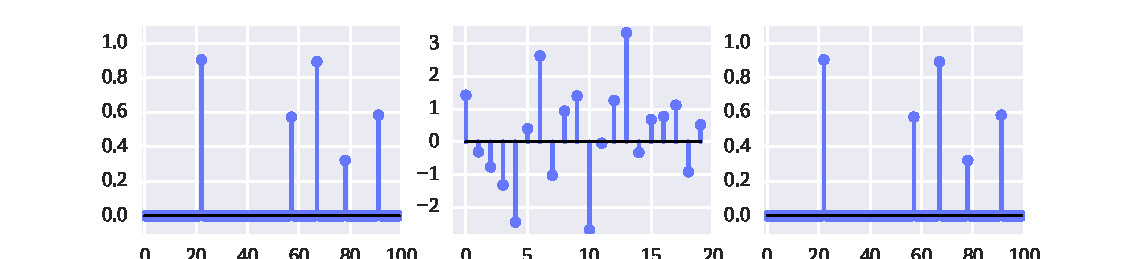
\includegraphics[width=\textwidth]{figs/figure_1h.pdf}
	\caption{\textit{Left}: The original $ 5 $-sparse vector $ x \in \R^{100} $. \textit{Center}: The sensed vector $ y \in \R^{20} $. \textit{Right}: Result of $ \ell_{1} $-minimization}
	\label{fig:l1min}
	\vspace{4pt}\hrule
\end{figure}





\subsection{Recasting \eqref{eq:P1} as a Linear Program} \label{sec:basisasLP}
Now that we have a tractable way of finding sparse solutions, we will look at one way to actually solve \eqref{eq:P1}. In this section we will see how one can use linear programming to do this. Linear programming (LP) is the study of problems on the form
\begin{equation}
	\maximize{\x\in\K^{N}} \c^{T}\x \quad \subjectto \A\x\leq\b~,~~ \x\geq\0
	\label{eq:LPgeneral}
\end{equation}
Thus, to use one of the algorithms developed for LP, we need to rewrite \eqref{eq:P1} as a linear program (ie, on the form \eqref{eq:LPgeneral}). 

In order to do this, three problems arise. Fist, we see from \cref{eq:LPgeneral} that LP problems do not take constraints on equality form, which is what we have in \eqref{eq:P1}. Second, LP problems only minimizes linear functions (ie, functions that can be written as a dot product between the solution vector and some constant vector). Absolute values, as we have in the $ \ell_{1} $ norm, can not be described this way. Third, a general LP problem requires all values in $ \x $ be non-negative. This is not a constraint we have in \eqref{eq:P1}.

We begin by addressing the first issue. This can be quite easily solved by observing that an equality constraint can be rewritten as two inequality constraints like so:
\[
	\A\z = \y \iff \A\z \leq \y \text{ and } \A\z \geq \y
\]

The second issue is a common one in LP. Thus there are also common ways to work around it. One popular way of doing this is to introduce new variables $ t_{i} $ for $ i \in \index{N} $ such that $ \abs{z_{i}} \leq t_{i} $ for all $ i $. Thus, 
\[ 
	\minimize{\z\in\Cx^{N}} \sum_{i=1}^{N} \abs{z_{i}}
\]
can be rewritten as
\[ 
	\minimize{\z,\mathbf{t} \in \Cx^{N}} \sum_{i=1}^{N}t_{i} \quad \subjectto \abs{z_{i}} \leq t_{i} \text{ for all } i \in \indexset{N}
\]
we can then rewrite the constraints as
\[
	\begin{array}{r l}
		z_{i} - t_{i} & \leq 0\\
		- z_{i} - t_{i} & \leq 0
	\end{array}
	\quad\text{for all } i \in \indexset{N}
\]
to arrive at the standard LP form. The $ t_{i} $'s are clearly non-negative since they are defined to be greater than or equal to an absolute value. 

The third issue is also a quite common one in LP. We now have two decision vectors, $ \z  $ and $ \mathbf{t} $, where the elements of $ \z $ does not need to be non-negative. We will solve this by introducing two new decision vectors $ \z_{+} $ and $ \z_{-} $, which will replace $ \z $ in the problem formulation. 

We define $ \z_{+} $ and $ \z_{-} $ as follows:
\[ 
	(\z_{+})_{i} = \twopartdef{z_{i}}{\text{if } z_{i} > 0}{0}{\text{otherwise}}
	\quad
	(\z_{-})_{i} = \twopartdef{-z_{i}}{\text{if } z_{i} < 0}{0}{\text{otherwise}}
\]
It is clear that $ \z = \z_{+} - \z_{-} $, it is also clear that $ \z_{+}, \z_{-} \geq \0 $. Substituting in $ \z_{+} - \z_{-} $ for $ \z $ in the original problem will then solve this issue. 

A final issue is that general LP problems concerns maximization problems, however \eqref{eq:P1} is a minimization problem. This is easily solved by observing that minimizing a function $ f $ is equivalent to maximizing $ -f $.

Combining all of the above we arrive at the LP formulation of basis pursuit:
\begin{equation}
%	\tag{P$_{1(LP)}$}
	\begin{array}{r r l l}
		\maximize{} & -\sum_{i=1}^{n} t_{i}         &          &  \\
		 \subjectto & \A\z_{+} - \A\z_{-}           & \leq \y  &  \\
		            & -\A\z_{+} + \A\z_{-}          & \leq -\y &  \\
		            & \z_{+} - \z_{-} - \mathbf{t}  & \leq \0  &  \\
		            & -\z_{+} + \z_{-} - \mathbf{t} & \leq \0  &  \\
		            & \z_{+}, \z_{-}, \mathbf{t}    & \geq \0   &
	\end{array}
\end{equation}
Thus, we can use all the celebrated algorithms for Linear Programming to solve \eqref{eq:P1}, such as the Simplex method, or various interior point methods \cite{vanderbei14linprog}.










\section{Good Sensing Matrices}
\label{sec:goodmatrices}
In this section we will look at the minimum number of measurements required, as well as some of the features we want our sensing matrix $ \A $ to possess, in order to ensure that basis pursuit works well. 

We will start by looking at how we can ensure unique $ s $-sparse solutions to the $ \ell_{1} $-minimization. Then we will look at how we can make sure that the solution to \eqref{eq:P1}, which is the problem we will solve in practice, is in fact the solution to \eqref{eq:P0}, which is the problem we actually want to solve. Finally we will look at which matrices will perform well with the different recovering algorithms used.





\subsection{Minimum Number of Measurements}
\label{sec:minimum_measurements}
In this section we will look at how many measurements we need in order to ensure that \eqref{eq:P0} has only one $ s $-sparse solution. We begin by stating the main result of this section:
\begin{theorem}
	\label{thm:minimum_measurements}
	If $ \set{\z \in \Cx^{N} \st \A\z = \A\x, \norm{\z}_{0} \leq s}  = \set{\x} $, that is, $ \x $ is the unique $ s $-sparse solution to \eqref{eq:P0}, then the number of measurements $ m $ must satisfy $ m \geq 2s $.
\end{theorem}

Before proving this theorem, we need the following lemma:
\begin{lemma}
	\label{lemma:uniquesol_linind}
	Every $ s $-sparse vector $ \x $ is the unique $ s $-sparse solution to \eqref{eq:P0} with $ \y = \A\x $ if and only if every set of $ 2s $ columns of $ \A $ is linearly independent.
\end{lemma}

We will not prove \cref{lemma:uniquesol_linind} in this report, but a proof can be found in \cite[Theorem~2.13]{foucart13intro}. We are now ready to prove the main result:
\begin{proof}[Proof of \cref{thm:minimum_measurements}]
	Assume that it is possible to uniquely recover any $ s $-sparse vector $ \x $ from the knowledge of its measurement vector $ \y = \A\x $. Then, by \cref{lemma:uniquesol_linind}, we have that every set of $ 2s $ columns of $ \A $ must be linearly independent. This implies that $ \rank \A \geq 2s $. From elementary linear algebra we know that the rank of a matrix can not be bigger that the number of rows, hence $ \rank \A \leq m $. Combining this, we get that
	\[
		2s \leq \rank \A \leq m
	\]
	which concludes the proof.
\end{proof}





\subsection{The Null Space Property}
\label{sec:NSP}
So far, we have only looked at the intuitive reasoning of why $ \ell_{1} $-minimization works well to find the $ \ell_{0} $-minimum. In this section we will formalize this relationship using the \textit{Null Space Property} (often abbreviated NSP). It can be shown that, for the NSP, the real and complex case are equivalent (for a formal statement and proof, see Theorem~4.7 in \cite{foucart13intro}). Hence we will state the definitions and results for a field $ \K $, which can be either $ \R $ or $ \Cx $. The NSP is defined as follows:

\begin{definition} \label{def:NSP}
	A matrix $ \A \in \K^{m\times N} $ is said to satisfy the \textit{null space property} relative to a set $ S \subset \indexset{N} $ if
	\[ 
		\norm{\v_S}_1 < \norm{\v_{\overline{S}}}_{1} \quad \forall ~ \v \in \ker \A \setminus \set{\0}
	\]
	It is said to satisfy the null space property of order $ s $ if it satisfies the null space property relative to any set $ S \subset \indexset{N} $ with $ \abs{S} \leq s $
\end{definition}

The definition of the NSP might seem a bit arbitrary, but as we will soon see, the NSP is directly connected to the success of basis pursuit. We begin by stating our first theorem on the NSP:

\begin{theorem}
	\label{thm:NSP_to_basis_special}
	Given a matrix $ \A \in \K^{m \times N} $, every vector $ \x \in \K^{N} $ supported on a set $ S $ is the unique solution to \eqref{eq:P1} with $ \y = \A\x $ if and only if $ \A $ satisfies the NSP relative to $ S $. 
\end{theorem}

\begin{proof}
	Proving equivalence amounts to proving two implications. We will begin by proving that if a vector $ \x $ supported on $ S $ uniquely solves \eqref{eq:P1}, then $ \A $ satisfies the NSP relative to $ S $.
	
	Given an index set $ S $, assume that every vector $ \x \in \K^{N} $ supported on $ S $ is the unique solution to
	\[
		\minimize{\z \in \Cx^{N}} \norm{\z}_1
		\subjectto \A\z = \A\x
		\tag{P$_1$}
	\]
	Since $ \ker\A $ is a subspace of $ \K^{N} $, it is clear that for any $ \v \in \ker\A\setminus\set{0} $, the vector $ \v_{S} $ is the unique solution to 
	\begin{equation}
		\label{eq:nspproofminprob}
		\minimize{\z \in \Cx^{N}} \norm{\z}_1
		\subjectto \A\z = \A\v_{S}
	\end{equation}
	Because $ \v \in \ker\A $, we have that $ \A\v = \0 $, which means that $ \A(\v_{S} + \v_{\overline{S}}) = \0 $, giving us that $ \A(-\v_{\overline{S}}) = \A\v_{S} $. Hence it clear that $ -\v_{\overline{S}} $ is also a feasible solution to \eqref{eq:nspproofminprob}, but since $ \v_{S} $ is assumed to be the \textit{unique} optimal solution to \eqref{eq:nspproofminprob}, we get that $ \norm{\v_{S}}_{1} < \norm{-\v_{\overline{S}}}_{1} $. Since $ \norm{\cdot}_{1} $ is a norm, we have that $ \norm{-\v_{\overline{S}}}_{1} = \abs{-1}\norm{\v_{\overline{S}}}_{1} = \norm{\v_{\overline{S}}}_{1} $ from \cref{def:norm}. Thus, we arrive at the following inequality:
	\[
		\norm{\v_{S}}_{1} < \norm{\v_{\overline{S}}}_{1}
	\]
	This establishes the NSP for $ \A $, relative to $ S $.
	
	To prove the other implication, assume first that the NSP holds for $ \A $, relative to a given set $ S $. Let $ \x $ be a vector in $ \K^{N} $ supported on $ S $. Let $ \z \in \K^{N} $ be a vector that satisfies $ \A\x = \A\z $, and assume that $ \x \neq \z $. Our goal will be to show that $ \norm{\z}_{1} $ must be strictly bigger than $ \norm{\x}_{1} $, which will prove the uniqueness of the solution. 
	
	Define $ \v = \x - \z $. Since $ \A\x = \A\z $, we have that 
	\[
		\0 = \A\x - \A\z = \A(\x -\z) = \A\v
	\]
	This means that $ \v \in \ker\A $. Since $ \x\neq\z $, we also have that $ \v\neq \0 $. If we use the triangle inequality of norms, as well as the definition of $ \v $, we obtain
	\[
	      \norm{\x}_{1} 
		= \norm{\x - \z_{S} + \z_{S}}_{1}
		  \leq \norm{\x - \z_{S}}_{1} + \norm{\z_{S}}_{1}
		= \norm{\v_{S}}_{1} + \norm{\z_{S}}_{1}
	\]
	Now, using the assumption that $ \A $ satisfies the NSP relative to $ S $ we get the next inequality
	\[
		\norm{\v_{S}}_{1} + \norm{\z_{S}}_{1} < \norm{\v_{\overline{S}}}_{1} + \norm{\z_{S}}_{1}
	\]
	Using the definition of $ \v $ and $ \z $ again, we arrive at our final result:
	\[ 
		  \norm{\v_{\overline{S}}}_{1} + \norm{\z_{S}}_{1}
		= \norm{\x_{\overline{S}} - \z_{\overline{S}}}_{1} + \norm{\z_{S}}_{1}
		= \norm{- \z_{\overline{S}}}_{1} + \norm{\z_{S}}_{1}
		= \norm{\z}_{1}
	\]
	This proves that $ \norm{\x}_{1} < \norm{\z}_{1} $ for any $ \z \in \K^{N} $ satisfying $ \A\x = \A\z $ and $ \x \neq \z $. This establishes the required minimality of $ \norm{\x}_{1} $, and thus the uniqueness of the solution.
\end{proof}

\cref{thm:NSP_to_basis_special} is not that interesting by itself, but if we let the set $ S $ vary, it immediately yields a more general result:

\begin{corollary}
	\label{thm:NSP_to_basis}
	Given a matrix $ \A \in \K^{m \times N} $, every $ s $-sparse vector $ \x \in \K^{N} $ is the unique solution to \eqref{eq:P1} with $ \y = \A\x $ if and only if $ \A $ satisfies the NSP of order $ s $. 
\end{corollary}

Before we prove this result, we will give a small remark: \cref{thm:NSP_to_basis} shows that if $ \A $ satisfies the NSP of order $ s $, the $ \ell_{1} $-minimization strategy of \eqref{eq:P1} will actually solve \eqref{eq:P0} for all $ s $-sparse vectors.

\begin{proof}[Proof of \cref{thm:NSP_to_basis}]
	Assume every $ s $-sparse vector $ \x\in\K^{N} $ is the unique solution to \eqref{eq:P1}. Then, for every set $ S $ with $ \abs{S} \leq s $ we can find a vector $ \x'\in\K $ supported on $ S $ which is the unique solution to \eqref{eq:P1}. By \cref{thm:NSP_to_basis_special} we then have that $ \A $ must satisfy the NSP relative to $ S $. Since this is true for all $ S $ with $ \abs{S} \leq s $, $ \A $ must satisfy the NSP of order $ s $.
	
	Conversely, assume that $ \A $ satisfies the NSP of order $ s $. Then, from \cref{def:NSP}, for every set $ S $ with $ \abs{S} \leq s $ we have that $ \A $ satisfies the NSP relative to $ S $. From \cref{thm:NSP_to_basis_special} we have that a vector $ \x\in\K^{N} $ is supported on $ S $ only if it is the unique solution to \eqref{eq:P1}. Since this is true for any set $ S $ with $ \abs{S} \leq s $, it is true for any $ s $-sparse vector.
\end{proof} 








\subsection{Coherence}
\label{sec:coherence}
Now that we know the minimum number of measurements needed for obtaining unique solutions, and the properties of $ \A $ needed to ensure that the solution to \eqref{eq:P1} is in fact the solution to \eqref{eq:P0}, we can start looking at how well the recovering algorithms will perform. In this section we will look at how the notion of \textit{coherence} can help us distinguish between matrices that will perform well with the different recovering algorithms, and which that will not. 

We want our reconstruction of $ \x $ to be fast and reliable. Since the $ i $'th element of our measurement vector $ \y $ is the inner product between the row $ i $ of $ \A $ and $ \x $, it makes intuitive sense that the columns of $ \A $ should be as ``scattered'' as possible. This leads us to the definition of coherence: 

\begin{definition}
	Let $ \A \in \Cx^{m\times N} $ be a matrix with $ \ell_{2} $-normalized columns $ \a_{1}, \a_{2}, \ldots, \a_{N} $. The \textit{coherence} $ \mu $ of $ \A $ is defined as
	\[
		\mu = \max_{1\leq i \neq j \leq N} \abs{\inner{\a_{i}}{\a_{j}}}
	\]
\end{definition}

It is worth noting that the coherence of a matrix $ \A $ is $ 0 $ if and only if $ \A $ is orthogonal. This agrees well with the intuitive approach discussed above. However, since compressive sensing deals with situations where $ m < N $, this will never be the case for any of the matrices we will look at. 

The question now becomes, how low can the coherence get? We know that we will never reach a coherence of $ 0 $, but how close can it be? The next lemma gives us a lower bound on the coherence:

\begin{lemma} \label{thm:welchbound}
	The coherence $ \mu $ of a matrix $ \A \in \K^{m \times N} $ with $ \ell_{2} $-normalized columns satisfies the following inequality:
	\[
		\mu \geq \sqrtl{\dfrac{N-m}{m(N-1)}}
	\]
\end{lemma}

\noindent This bound is often called the \textit{Welch bound}. The proof for this Lemma is rather technical, and will therefore be omitted from this report. A complete proof for \cref{thm:welchbound} can be found in \cite[Theorem~5.7]{foucart13intro}.

\todo[inline]{Eksempel med matriser med lav koherens?}







\section{Sparsity in the Real World}
\subsection{Compressibility}
The general framework developed in \cref{sec:goodmatrices} is designed for \textit{sparse} vectors without any errors. What if our signal is almost sparse, but not quite? Or what if the sampled signal is slightly distorted? In this section we will briefly cover how we can extend the theory presented in \cref{sec:goodmatrices} to cover such cases.

In order to answer this precisely we first need to specify what we mean with \textit{almost sparse}. This is where the notion of compressibility comes in. A compressible vector is a vector where most entries is \textit{almost} zero. To more precisely define a compressible vector, we must first define what we mean by almost zero:
\begin{definition} \label{def:compressibility}
	For any $ p > 0 $, the $ \ell_{p} $-error of best $ s $-term approximation to a vector $ \x \in \Cx^{N} $ is defined by
	\(
		\sigma_{s}(\x)_{p} = \inf \set{\norm{\x - \z}_{p} : \z \text{ is } s\text{-sparse}}
	\)
\end{definition}

We say that a vector $ \x $ is $ s $-compressible if $ \sigma_{s}(\x)_{1} $ is small. The second potential issue we will cover is when our measured vector $ \y $ contains some noise, such that $ \A\x \approx \y $. If the distance between the distorted measurements $ \y $ and the real, unbiased signal $ \A\x $ is bounded by a parameter $ \epsilon $, we can rewrite the approximation constraint as $ \norm{\A\x - \y}_{2} < \epsilon $. This motivates the following variant of basis pursuit:
\begin{equation}
	\tag{P$_{1, \epsilon}$}
	\label{eq:P1eps}
	\minimize{\z\in\Cx^{N}} \quad\subjectto \norm{\A\z - \y}_{2} \leq \epsilon
\end{equation}
It can be shown that if the sensing matrix exhibits a strengthening of the NSP called \textit{robust NSP}, the error made by solving \eqref{eq:P1eps} is bounded by a weighted sum of $ \sigma_{s}(\x)_{1} $ and $ \epsilon $ \cite[Section~4.3]{foucart13intro}.



\subsection{Achieving Sparsity or Compressibility}
So far we have just assumed our solution vector $ \x $ to be sparse or compressible. However, most real life signals are rarely sparse. Images are usually not mostly black, and songs are usually not mostly silence. Hence, we need some way to represent natural signals in a sparse way. 

We will achieve this by applying what is known as a \textit{sparsifying transform}. Many such transforms exists, but in this report we will consider the \textit{Haar wavelet transform} as an example. The Haar wavelet is by far not the most efficient sparsifying transform, but it is quite understandable, which is why we have chosen it. 

The key idea in a wavelet transform is to take some object, expressed in a high resolution wavelet basis, and express it in terms of a lower resolution basis, and a detail basis. In the specific case of the Haar wavelet, those functions are defined as follows:
\[
	\phi(t) = \twopartdef{1}{\text{if } 0\leq t < 0}{0}{\text{otherwise}}
	\quad
	\psi(t) = \threepartdef{1}{\text{if } 0\leq t < 1/2}{-1}{\text{if } 1/2 \leq t < 1}{0}{\text{otherwise}}
\]
By shifting and scaling those functions we get a basis for the low resolution space (from the $ \phi $'s) and the detail space (from the $ \psi $'s). Since a digital image is piecewise linear in every pixel, it is clear that a digital image of size $ n \times n $ is in the $ n \times n $ dimensional high resolution resolution space for the Haar wavelet.

The Haar Discrete Wavelet Transform (Haar DWT) is essentially a change of coordinates from the higher resolution wavelet basis basis, to a lower resolution and detail basis. \cref{fig:dwt_sparsifying} illustrates what happens when the DWT is applied to an image. The upper left corner of the resulting image is the low resolution space. This is usually not any sparser or more compressible than the original image. However, in the upper right, lower left and lower right corners we see the detail space. This is highly compressible, and it is also clear that the total compressibility of the image has increased (ie, number of non-zero components has decreased). We will denote the corresponding matrix to this change of coordinates by $ \mathbf{\Psi} $. 

\begin{figure}[t]
	\centering
	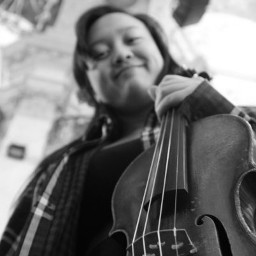
\includegraphics[width=0.47\textwidth]{figs/lily.jpg}
	\hspace{.039\textwidth}
	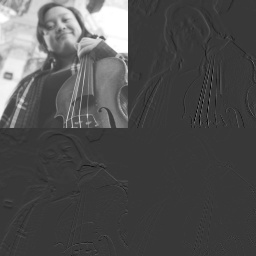
\includegraphics[width=0.47\textwidth]{figs/lily_wavelet.jpg}
	\caption{\textit{Left:} the original image of Lily. \textit{Right:} the image after a 1-level discrete wavelet transform using the Haar wavelet. In this example, we have used the 2D DWT implementation provided in \cite{ryan16applinalg}.}
	\label{fig:dwt_sparsifying}
	\vspace{4pt}\hrule
\end{figure}

We could assume that this change of coordinates have been done prior to the sensing, so that our solution vector $ \x = \mathbf{\Psi}\x' $ is sparse. Here $ \x' $ is the underlying non-sparse solution. However, we will instead include the change of coordinates in our sensing matrix $ \A $. Hence the sensing matrix becomes the following product:
\begin{equation}
	\label{eq:sensingmatrix_composition}
	\A = \mathbf{P}_{\Omega}\mathbf{\Phi}\mathbf{\Psi}^{-1}
\end{equation}
Here, $ \mathbf{P}_{\Omega} $ is a matrix describing the down-sampling, $ \mathbf{\Phi} $ denotes the sampling pattern used, and $ \mathbf{\Psi} $ is the basis in which $ \x $ is sparse. Typical choices include letting $ \mathbf{\Psi} $ be some wavelet basis, letting $ \mathbf{\Phi} $ be rows from the discrete Fourier matrix, and letting $ \mathbf{P}_{\Omega} $ pick out the first $ n $ rows.

This means that solving \eqref{eq:P1} results in a recovered vector $ \z $ also expressed in the $ \mathbf{\Psi} $-basis. To recover our real non-sparse vector $ \z' $ we would then have to apply the reversed change of coordinates:
\[
	\z' = \mathbf{\Psi}^{-1}\z 
\]
Since the columns of $ \mathbf{\Psi} $ form a basis, we know that the inverse $ \mathbf{\Psi}^{-1} $ exists by the Invertible Matrix Theorem.
%\cite[Theorem~2.8m]{lay16linearalgebra}


For ease of notation, we will simply refer to the sampling matrix as $ \A $, even though we think of it as a product of multiple matrices. The concepts we discussed earlier in \cref{sec:goodmatrices} will apply to this product $ \A $. We will also note that we will later use $ \mathbf{\Phi} $ to denote a matrix generated from training images. This is a different matrix, and should not be confused with the sampling pattern here. 





